%template for producing Interface-format articles using LaTeX. 
%Tim Hesterberg, MathSoft (formerly Statistical Sciences), 12 Sept 96
%from IEEE example by Matthew Ward, Worcester Polytechnic Institute. 
%updated for CD-ROM format (as of Interface 2001) by 
%Juergen Symanzik, Utah State University (symanzik@sunfs.math.usu.edu), Aug 2001
%Please send comments to symanzik@sunfs.math.usu.edu or timh@statsci.com.
\documentclass[10pt]{article}
\pagestyle{empty}
\usepackage{hyperref}
\usepackage{harvard}
\usepackage{amsthm,amsfonts,amsmath}
\usepackage{enumitem}
%\usepackage[pdftex]{graphicx}%%for Pdftex
\usepackage{graphicx}%%for Latex
\usepackage{multirow}
\usepackage{bbm}
\usepackage{amssymb}
\usepackage{amsthm}
\usepackage{url}
\usepackage{mathrsfs}
\usepackage{appendix}
%\usepackage[pdftex]{graphicx}
%\usepackage{subfigure}
%\usepackage{multicol}
%\usepackage{color}
\usepackage{algorithm}
\usepackage{algorithmic}
\usepackage{setspace}

%set dimensions of columns, gap between columns, and paragraph indent 
\setlength{\textheight}{8.5in}
\setlength{\textwidth}{5in}
\setlength{\headheight}{0cm}
\setlength{\headsep}{0cm}
%\setlength{\footheight}{0.0in}
\setlength{\parindent}{1pc}

%macro
%%%%%%%%%%%%%%%%%%%%%%%%%%%%%%%%%%%%%%%%%%%%%%%%%%%%%%%%%%%%%%%%%%%%%%%%%
\hyphenation{con-tin-u-ous-time con-tin-u-ous bank-rupt-cy}
\hyphenation{Lebes-gue} \hyphenation{ter-mi-nol-o-gy}
%%%%%%%%%%%%%%%%%%%%%%%%%%%%%%%%%%%%%%%%%%%%%%%%%%%%%%%%%%%%%%%%%%%%%%%%%
\newcommand{\bbr}{\mathbb{R}}  %black board bold \mathbb{R}
\newcommand{\bbn}{\mathbb{N}}
\newcommand{\bbp}{\mathbb{P}}
\newcommand{\bY}{\mathbf{Y}}
\newcommand{\mun}{\lceil \mu n \rceil}
\newcommand{\etan}{\lceil \eta n \rceil}
\newcommand{\bbq}{\mathbb{Q}}
\newcommand{\wQ}{\widetilde{\bbp}}%change per Prof. Lai's request to alleviate confusion
\newcommand{\wq}{\widetilde{p}}%change per Prof. Lai's request to alleviate confusion
\newcommand{\wY}{\widetilde{Y}}
\newcommand{\wX}{\widetilde{X}}
\newcommand{\ow}{\overline{w}}
\newcommand{\wht}{\widehat}
\newcommand{\var}{\ensuremath{\mathbb Var}}
\newcommand{\wbY}{\widetilde{\bY}}
\newcommand{\abs}[1]{\lvert#1\rvert}
\newcommand{\D}{\mathbb{D}}
\newcommand{\G}{\mathbb{G}}
\newcommand{\bbe}{\mathbb{E}}
\newcommand{\F}{\mathbb{F}}
\newcommand{\HH}{\mathbb{H}}
\newcommand{\bbj}{\mathbb{J}}
\newcommand{\bbz}{\mathbb{Z}}
\newcommand{\bbs}{\mathbb{S}}
\newcommand{\C}{\mathbb{C}}
\newcommand{\bu}{\mathbf{u}}
\newcommand{\bx}{\mathbf{x}}
\newcommand{\fn}{\footnote}
\newcommand{\ci}{\citeasnoun}
\newcommand{\om}{\omega}
\newcommand{\la}{\lambda}
\newcommand{\tla}{\tilde{\lambda}}
\newcommand{\doth}{f}
\renewcommand{\labelenumi}{\roman{enumi}}
\newcommand{\ps}{P}
\newcommand{\pss}{\ensuremath{\mathbf{p}}} %small boldface
\newcommand{\pmq}{\ensuremath{\mathbf{Q}}}
\newcommand{\pmqs}{\ensuremath{\mathbf{q}}}
\newcommand{\pas}{P-a.s. }
\newcommand{\pasm}{P\mbox{-a.s. }}
\newcommand{\asm}{\quad\mbox{a.s. }}
\newcommand{\cadlag}{c\`adl\`ag }
\newcommand{\fil}{\mathcal{F}}
\newcommand{\gcal}{\mathcal{G}}
\newcommand{\hcal}{\mathcal{H}}
\newcommand{\jcal}{\mathcal{J}}
\newcommand{\pcal}{\mathcal{P}}
\newcommand{\ecal}{\mathcal{E}}
\newcommand{\bcal}{\mathcal{B}}
\newcommand{\ical}{\mathcal{I}}
\newcommand{\scal}{\mathcal{S}}
\newcommand{\ncal}{\mathcal{N}}
\newcommand{\lcal}{\mathcal{L}}
\newcommand{\kcal}{\mathcal{K}}
\newcommand{\acal}{\mathcal{A}}
\newcommand{\mcal}{\mathcal{M}}
\newcommand{\rcal}{\mathcal{R}}
\newcommand{\tcal}{\mathcal{T}}
\newcommand{\ti}{\times}
\newcommand{\we}{\wedge}
\newcommand{\be}{\begin{equation}}
\newcommand{\ee}{\end{equation}}
\newcommand{\bew}{\begin{equation*}}
\newcommand{\eew}{\end{equation*}}
\newcommand{\uK}{\underline K}
\newcommand{\oK}{\overline K}
\renewcommand{\th}{\tilde{h}}
\newcommand{\imp}{\eta}
\newcommand{\xbar}{\overline{X}}
\newcommand{\Xij}{X_{i,j}}
\newcommand{\f}{\left}
\newcommand{\g}{\right}
\newcommand{\naiveest}{\wht{\sigma^2_n}}
\newcommand{\deltaest}{\wht{\sigma^2_d}}

%theorem style
\newtheorem{thm}{Theorem}
\newtheorem{cond}[thm]{Condition}
\newtheorem{defi}[thm]{Definition}
\newtheorem{algo}[thm]{Algorithm}
\newtheorem{prop}[thm]{Proposition}
\newtheorem{corollary}[thm]{Corollary}
\newtheorem{lem}[thm]{Lemma}
\newtheorem{rem}[thm]{Remark}
\newtheorem{ex}[thm]{Example}
\newtheorem{ass}[thm]{Assumption}

\begin{document}

%don't want date printed
\date{}

%make title bold and 14 pt font (Latex default is non-bold, 16pt) 
\title{\Large\bf Finite User Pool Effect in Two Sample t-test of Controlled Experiments on the Web}

%for single author (just remove % characters)
\author{Shaojie Deng \\
  Microsoft \\
  Redmond, WA, 98052}

%for two authors (this is what is printed)
%\author{\begin{tabular}[t]{c@{\extracolsep{8em}}c}
%  I. M. Author  & M. Y. Coauthor \\
% \\
%  My Department & Coauthor Department \\
%  My Institute & Coauthor Institute \\
%  City, STATE~~zipcode & City, STATE~~zipcode
%\end{tabular}}

\maketitle

%So first page doesn't have a page number
\thispagestyle{empty}

\subsection*{Abstract}
i.i.d. assumption is a basic assumption made in the application of two sample t-test in practice. In this paper, we show that when this assumption is not true and the sampling scheme is replaced by sample without replacement from a finite pool, the variance estimator assuming i.i.d. samples overestimates the variance. The overestimating effect is small or negaligile when the sample size is small relative to the finite pool size. However, the results in this paper is relavent to controlled experiment on the web because the capability of conducting controlled experiments using a large proportion of the whole web users. 

\subsection*{Keywords}
Controlled experiment, Experimentation, A/B testing, t-test, Variance estimation. 


\section{Introduction}
For centuries people have been looking for ways to evaluate ideas. Controlled experiment, also called randomized test or A/B test has long established its importance as the methodology to establish a causal relationship. This paper will be focused on controlled experiment on the web. An obvious difference between controlled experiment on the web and other types of controlled experiment (for example, clinical trials) is that it is easy to collect data on web at low cost. In other words, web provides an unprecedented opportunity for us to use the power of controlled experiment to test and evaluate ideas quickly. It is our strong belief that unlocking the large amount of data on the web using the right methodology to analyze it is the key toward a data driven philosophy, and controlled experiment has successfully set a standard in the industry.  There are already many publications in the literature on controlled experiment. For a good and thorough survey on how to run web experiments, see \ci{expsurvey}.  Most of the works in the literature are focused on practical issues and best practices. To the author's knowledge few of them have been contributed on the underlying statistical methods. Part of the reason is that the related statistical method --- the widely used two sample t-test are so well known, under i.i.d assumptions. In this paper, we show that when this assumption is modified in light of the fact that the total user pool is finite and sampling unit is not exactly i.i.d, the statistical analysis is more subtle and the results are different. 

To better convey the idea, we need to introduce some terminology. A \emph{experiment unit} is the unit on which the randomization is applied. The most commonly used experiment unit is user or its surrogate such as cookie. Page view has also been used in practice; see \ci{googlesurvey}.  A \emph{metric} is an statistic that stands for some concept the experiment designer wants to evaluate. Common metrics includes clicks per user, sessions per user, click through rate, coverage rate, etc. A metric is naturally associated with an \emph{analysis unit}. For example, per user metric such as clicks per user has the analysis unit user. Click through rate and coverage rate use page view as the analysis unit. The analysis unit associated with a metric is also called the \emph{level} of the metric. The most important two types of metrics are user level metrics and page view level metrics.  A \emph{measurement} is an observation on a analysis unit. For example, the number of clicks of user $i$ on page view $j$ is a page view level measurement. It can be further rolled up (summed up) to user $i$'s total number of clicks, which is a user level measurement. 

In the following, we will focus on the case that user is the experiment unit.  The general procedure of the statistical testing in web controlled experiment can be described as follows. Suppose we are interested in a metric $S$. After data was collected, we can calculate the value of this metric for both control group and treatment group, denoted by $S_c$ and $S_t$. Under the assumption that user level measurement are i.i.d., central limit theorem guarantees that $S_t$ and $S_c$ is asymptotically normal and we can estimate the variance of $S_t$, $S_c$. Standard two-sample t-test can then be applied because $\frac{S_t-S_c}{\var(S_t-S_c)} =\frac{S_t-S_c}{\var (S_t)+\var (S_c)}$ is asymptotically normal. The central player of this approach, is therefore to estimate the variances $\var S_t$ ( and $\var S_c$). 

The assumption that user level measurements are i.i.d. bears close examination. Because each user is a unique human being and the total number of users in the universe is a finite number, if we sample a fixed percentage $x$ of total users for control or treatment, this sampling is sampling without replacement and theoretically it cannot be independent.\footnote{This will be rigorously addressed in Section \ref{finitecase}.} But on the other hand, the i.i.d. assumption has never been questioned because in most cases, we only sample a tiny portion of the total user pool and as the result, sampling without replacement and sampling with replacement does not differ to a degree that will change the result. For example, in clinical trial, the trial was only done to  a cohort of people, hundreds or thousands. Comparing to the total population on earth is in billion, it is safe to assert the i.i.d assumption and would actually be pedantic to question it. 

For controlled experiment on the web, however, unlike the case for clinical trial, we do have the capability of experimenting on \emph{all of the users that could show up}. It is not unusual to have a 50\%/50\% controlled experiment in which half of the total users received the control experience and the other half the treatment. For these cases, the finite user effect is no longer negligible and the variance calculation needs to be adjusted in light of this effect. In this paper, we show how the adjustment can be made from a simple formula. The adjusted variance estimate is smaller than the estimate under the i.i.d assumption. Therefore two sample t-test without this adjustment will be over conservative and losing power. To our knowledge, this problem has not been studied in previous publications and there are no related literatures. 

The following paper is organized as follows. We first introduce notation in Section \ref{notation}. In Section \ref{infcase},  asymptotic results on the variance of both page level metric and user level metric under the assumption of infinite user pool are presented. The main results of this paper are in Section \ref{finitecase}, where we exam the finite user pool effect and propose simple formula called Formula X for variance estimation for both page level and user level metric. Section \ref{simulation} presents simulation study that shows the performance of Formula X. Section \ref{conclusion} summarizes and concludes. 

\subsection{Notation}\label{notation}
Before going into the next section, we introduce notation and assumptions which will be consistently used through out this paper. Denote $n$ the total number of unique users. Let $X_{i,j}$ be the per-page measurement (e.g. number of clicks on the page) on user $i$'s $j^{th}$ page view and $X_{i,j}$ has mean $\mu_i$ and variance $\sigma_i^2$.  Denote $K_i$ the total number of page views from user $i$ and $N = \sum_{i=1}^n K_i$ be the total number of page views. We assume for any $i$, $X_{i,j},j=1,\dots,K_i$ are i.i.d. and uniformly bounded above by some finite constant.  But we allow $(\mu_i,\sigma_i^2)$ to differ from user to user. We also assume $K_i,i=1,\dots,n$ are i.i.d. and independent of $(\mu_i,\sigma_i^2),i=1,\dots,n$. This last assumption may not be true in practice and need to be checked case by case. We have checked this assumption for some key metrics of web experiments using empirical data and this assumption is reasonable. 

\section{Infinite User Pool Case}\label{infcase}
In this section, we assume there are infinite number of users in the universe. A direct impact of this assumption is that we can assume $(\mu_i,\sigma_i^2),i=1,\dots,n$ are i.i.d. realizations from some distribution. Note that $(\mu_i,\sigma_i^2)$ represents the user effect on the page level measurement $X_{i,j}$, and this model is a random effect model where the user effect is the random effect. We will derive the variance of the page level metric as well as that of the user level metric and also provide some theoretical results on some common estimators of the variance. Although the results might seem to be irrelevant to the topic of this paper, we present these results for the following reasons. First, they are interesting results that reveals important insights of the variances that are crucial for t-tests. Secondly, they provide the building blocks for Section \ref{finitecase} where we present the main results of this paper. 

\subsection{Page Level Metrics}
A page level metric can be denoted by:
\begin{align*}
\xbar= \frac{\sum_{i=1}^n\sum_{j=1}^{K_i} X_{i,j}}{N}.
\end{align*}
To estimate the variance of $\xbar$, it is tempting to treat page level metrics $X_{i,j}$, $j=1,\dots,K_i$, $i=1,\dots,n$, as i.i.d. and $\xbar$ under this assumption is an average of i.i.d. samples so the variance of $\xbar$ can be easily estimated by
\begin{align*}
\frac{1}{N^2} \Bigl (\sum_{i=1}^n \sum_{j=1}^{K_i} (X_{i,j}-\overline{X})^2 \Bigr ).
\end{align*}
This estimator, which we call the \emph{naive} estimator,  is not consistent because unlike the fixed effect model, where the only randomness is from the noise of $X_{i,j}$. In our model the user effect $(\mu_i,\sigma_i^2)$ are also a random sample from a distribution. Nevertheless, it is true in our model that the user level measurement $(\sum_{i=1}^{K_i} X_{i,j}, K_i),i=1,\dots,n$ are i.i.d. By letting $Y_i = \sum_{i=1}^{K_i} X_{i,j}$ and express $\xbar$ as $\sum_{i=1}^n Y_i / \sum_{i=1}^n K_i$, it is then a straightforward application of the delta method to get an asymptotically consistent estimator for $\var \xbar$:
\begin{align*}
\frac{1}{n} \Bigl\{ \frac{1}{\wht{\bbe K_i}^2}\wht{\var Y_i} + \frac{\wht{\bbe Y_i}^2}{\wht{\bbe K_i}^4}\wht{\var K_i} - 2\frac{\wht{\bbe Y_i}}{\wht{\bbe K_i}^3} \wht{Cov(Y_i,K_i)} \Bigr\} 
\end{align*}
where these ``hatted'' quantities are the sample mean, variance or covariance. 

For asymptotic analysis, we will let $n\to \infty$ (so $N\to \infty$ a.s.). To normalize the naive estimator and delta method estimator, we multiply them by $n$ so that they will converge to some nonzero numbers.  We introduce the normalized naive estimator 
\begin{align}
\wht{\sigma^2_n} = n\frac{1}{N^2} \Bigl (\sum_{i=1}^n \sum_{j=1}^{K_i} (X_{i,j}-\overline{X})^2 \Bigr ).
\end{align}
and the normalized delta method estimator
\begin{align}
\wht{\sigma^2_d} = \frac{1}{\wht{\bbe K_i}^2}\wht{\var Y_i} + \frac{\wht{\bbe Y_i}^2}{\wht{\bbe K_i}^4}\wht{\var K_i} - 2\frac{\wht{\bbe Y_i}}{\wht{\bbe K_i}^3} \wht{Cov(Y_i,K_i)}
\end{align}
A natural question to ask is how biased is the naive estimator $\naiveest$ relative to the true normalized variance $n\var \xbar$. This is answered in the following theorem.
\begin{thm}\label{thm1.1}
Let $C = \frac{\bbe K_i^2}{(\bbe K_i)^2}$.  Then, as $n\to \infty$,
\begin{align}
n\var\xbar &\to C \var(\mu_i) + \bbe(\sigma^2_i)/\bbe (K_i)\label{truevar} \\
\deltaest & \to  C \var(\mu_i) + \bbe(\sigma^2_i)/\bbe (K_i)\label{deltalim}  \\
\naiveest & \to  \frac{1}{\bbe(K_i)} (\var(\mu_i)+\bbe(\sigma_i^2))\label{naivelim}.
\end{align}
Let $\rho:= \var(\mu_i)/(\var(\mu_i)+\bbe(\sigma^2_i))$ be the user effect coefficient(variances that explained by between user variation), then
\begin{align}
\frac{n\var (\xbar)}{\naiveest} \to  (\bbe(K_i)C - 1)\rho +1.
\end{align}
The convergence in \eqref{deltalim} and \eqref{naivelim} are  in probability. 
\end{thm}

\begin{proof}[Proof of Theorem \ref{thm1.1}.]
\eqref{deltalim} follows directly from the property of the delta method. To prove \eqref{truevar}, we first apply conditional variance formula by conditioning on $(\mu_i,\sigma_i^2, K_i, i=1,\dots,n)$. This gives
\begin{align*}
&\var \xbar =  \var  \Bigl( \bbe\Bigl(   \frac{\sum_{i=1}^n\sum_{j=1}^{K_i} X_{i,j}}{N} \Big| K_i,\mu_i,\sigma_i^2,  i=1,\dots,n\Bigr) \Bigr) \\
+&\bbe \Bigl(\var \Bigl( \frac{\sum_{i=1}^n\sum_{j=1}^{K_i} X_{i,j}}{N} \Big | K_i,\mu_i,\sigma_i^2,  i=1,\dots,n\Bigr)\Bigr) \notag\\
=&\var \Bigl(\frac{1}{N}\sum_{i=1}^n K_i \mu_i \Bigr)+\bbe \Bigl(\frac{1}{N^2}\sum_{i=1}^n K_i \sigma^2_i \Bigr).
\end{align*}
Let  $w_i = K_i/\sum_{i=1}^n K_i = K_i/N$. Since $K_i$ independent of $(\mu_i, \sigma^2_i)$ and $N/n \to \bbe {K_i}$ as $n\to \infty$, we can further simplify the right hand. First, by applying iterative expectation(frist conditioning on $w_1,\dots, w_n$), we have  
\begin{align}
n \bbe \Bigl(\frac{1}{N^2}\sum_{i=1}^n K_i \sigma^2_i \Bigr)  = \sum_{i=1}^n \bbe\Bigl( \frac{n}{N} w_i\sigma^2_i \Bigr) = \frac{1}{\bbe K_i}(\sum_{i=1}^n w_i)\bbe \sigma_i^2 = \frac{\bbe \sigma_i^2}{\bbe K_i} \label{withinterm}
\end{align}
where the second equality is by bounded convergence theorem(since $N/n \to \bbe {K_i}$ and $\sum w_i\sigma^2_i$ bounded) and the last equation is from $\sum w_i=1$. Since $(\mu_i, \sigma^2_i), {i=1,\dots, n}$ are i.i.d., 
\begin{align}
&n\var (\sum_{i=1}^n w_i \mu_i) = n\bbe (\var (\sum_{i=1}^n w_i \mu_i|w_1,\dots,w_n))+ n\var (\bbe (\sum_{i=1}^n w_i \mu_i|w_1,\dots,w_n)) \\
&=  n\bbe (\sum_{i=1}^n w_i^2 \var(\mu_i)) + n \var((\sum_{i=1}^n w_i)\bbe\mu_i ) = n\bbe(\sum_{i=1}^n w_i^2) \var (\mu_i) \label {betweenterm}
\end{align}
where the last equality is from the fact that the second term is $0$. By simple algebra, 
$n \sum_{i=1}^n w_i^2 =  \frac{\overline{K_i^2}}{\overline{K_i} \times \overline{K_i}}$, where $\overline{K_i^2}$ and $\overline{K_i}$ are sample mean of $K_i^2$ and $K_i$, respectively.
By strong law of large number, $\overline{K_i^2}\to \bbe K_i^2$ a.s., $\overline{K_i}\to \bbe K_i$ a.s., therefore $n \sum_{i=1}^n w_i^2 =  \frac{\bbe{K_i^2}}{(\bbe{K_i})^2}$ a.s. Combine this result with \eqref{withinterm} and \eqref{betweenterm}, we've proved \eqref{truevar}.

We now turn to the limit of $\naiveest$. 
\begin{align*}
 \naiveest &= n \frac{1}{N^2} \Bigl (\sum_{i=1}^n \sum_{j=1}^{K_i} (X_{i,j}-\overline{X})^2 \Bigr )= \frac{n}{N^2} \Bigl \{  \sum_{i=1}^n \sum_{j=1}^{K_i} X_{i,j}^2 - N \xbar^2 \Bigr\}\\
&\to   \lim_{n\to \infty} \Bigl(\frac{n^2}{N^2}\Bigr) \bbe \bigl(\sum_{j=1}^{K_i} \Xij^2 \bigr) -   \lim_{n\to \infty} \Bigl(\frac{n}{N}\Bigr) (\bbe \mu_i)^2 .
\end{align*}
The last limit is from $(1/n) \sum_{j=1}^{K_i} X_{i,j}^2 \to \bbe \bigl(\sum_{j=1}^{K_i} \Xij^2 \bigr)$ and $\xbar \to \bbe \mu_i$ a.s., both by the strong law of large number.
Using bounded convergence theorem and $N/n \to \bbe K_i$, and also $\bbe \bigl(\sum_{j=1}^{K_i} \Xij^2 \bigr)  = \bbe K_i \bbe X_{i,j}^2 = \bbe K_i (\bbe \mu_i^2 + \bbe \sigma_i^2)$,
\eqref{naivelim} follows.
\end{proof}

\subsection{User Level Metrics}
A user level metric can be denoted by 
\begin{align*} 
\wX = \frac{\sum_{i=1}^n\sum_{j=1}^{K_i} X_{i,j}}{n} = \frac{\sum_{i=1}^n Y_i}{n}
\end{align*}
A consistent estimator for $n\var \wX$ is the sample variance of $Y_i$. The following theorem gives the formula of $n\var \wX$. 
\begin{thm}\label{thm1.2} 
As $n\to \infty$, 
\begin{align*}
n\var \wX \to \bbe K_i^2 \var \mu_i + (\bbe \mu_i)^2 \var K_i + \bbe K_i \bbe \sigma_i^2.
\end{align*} 
\end{thm}
This theorem is a special case of a more general theorem in Section \ref{finitecase}. We defer the proof to Section \ref{finitecase}.

\section{Finite User Pool Effect}\label{finitecase}
In this section, we consider the case that the number of users are finite, although the number can be very large. We label these users by index $i=1,\dots, M$ and suppose they have their own $(\mu_i,\sigma_i^2)$ fixed but unknown. For an on-line controlled experiment, we first sampled a portion $x$ of users from the $M$ total users without replacement where $0<x\le 1$.  wlog, in the following we let $n = xM$ and treat it as an integer. Note that because users are sampled without replacement, $(\mu_i,\sigma_i^2)$ of those $n$ sampled users are no longer i.i.d. The sampling without replacement scheme can be equivalently modeled as the following reshuffle scheme. Suppose we first shuffle the $(\mu_i,\sigma^2_i)_{i=1,\dots,M}$ and then relabel these from $1$ to $M$. We then select the first $i=1,\dots,n$  as the users that are sampled. The purpose of using this model is that we can still use index $i=1,\dots,n$ in the proof rather than introducing an additional layer of index $S_i$ denoting the index of the $i^{th}$selected user. 

We first study the limit of the normalized variance of a page level metric $\xbar$ and propose a consistent estimator in the following theorem:
\begin{thm}\label{thm2.1}
Let $C = \frac{\bbe K_i^2}{(\bbe K_i)^2}$.  As $n\to \infty$,
\begin{align}
n\var\xbar &\to (C-x) \var(\mu_i) + \bbe(\sigma^2_i)/\bbe (K_i)\label{truevar2} \\
\deltaest & \to  C \var(\mu_i) + \bbe(\sigma^2_i)/\bbe (K_i)\label{deltalim2}  \\
\naiveest & \to  \frac{1}{\bbe(K_i)} (\var(\mu_i)+\bbe(\sigma_i^2))\label{naivelim2},
\end{align}
where the measure for $(\mu_i,\sigma_i^2)$ are the law corresponding to sample one $(\mu_i,\sigma_i^2)$ from $(\mu_i,\sigma_i^2), i=1,\dots,M$. Moreover, 
\begin{align}\label{twoestimator}
\wht{\var \mu_i} = \frac{\deltaest-\naiveest}{\frac{\wht{\bbe Ki^2})}{\wht{\bbe K_i}^2}- \frac{1}{\wht{\bbe K_i}}},\quad
\wht{\bbe \sigma_i^2}  = \wht{\bbe K_i} \Bigl(\deltaest^2 -  \frac{\deltaest-\naiveest}{1- \frac{\wht{\bbe K_i}}{\wht{\bbe K_i^2}}}\Bigr)
\end{align}
are consistent estimator for $\var \mu_i$ and $\bbe \sigma_i^2$ respectively. Therefore a consistent estimator of $n\var \xbar$ is:
\begin{align*}
(\wht{C} - x) \wht{\var \mu_i} + \wht{\bbe \sigma_i^2}/\wht{\bbe (K_i)}= \deltaest - x \wht{\var \mu_i}. \tag{Formula X}
\end{align*}
\end{thm}

Theorem \ref{thm2.1} shows that under the finite user pool assumption, the normalized variance $n\var \xbar$ decreases linearly  as $x$ increases from $0$ to $1$. On one extreme, when $x$ close to 0, the distinction between sampling with replacement and sampling without replacement is so small that it is safe to treat $(\mu_i,\sigma_i^2)$ as i.i.d. just as in the case of infinite user pool case treated in Section \ref{infcase}. On the other extreme, when $x=1$, we have observed all the users in one group, the user effect is reduced because we will always have the same set of users (same set of $(\mu_i,\sigma_i^2), i=1,\dots,n)$. In controlled experiment, since we have at least two groups, we will not let $x$ close to 1. But there are cases that we allocated 50\% of traffic to both control and treatment group, corresponds to the case $x=0.5$. If we ignore the finite user pool effect, we will be using the delta method estimator $\deltaest$ to estimate the normalized variance, which by theorem \ref{thm2.1} is upward biased by a factor of $x \var \mu_i$. We name the consistent estimator Formula X where the ``X'' stands for its relationship with the parameter $x$ and also stands for the fact that this estimator is a hybrid of $\deltaest$ and $\naiveest$. 

\begin{proof}[Proof of Theorem \ref{thm2.1}.]
First note that the delta method estimator will converge to the limit of $n\var \xbar$ as if $(\mu_i,\sigma_i^2)$ were i.i.d. from the law corresponding to sample one $(\mu_i,\sigma_i^2)$ from $(\mu_i,\sigma_i^2), i=1,\dots,M$. In this case from Theorem \ref{thm1.1}, \eqref{deltalim2} follows. $\eqref{naivelim2}$ follows from a similar argument as in the proof of Theorem \ref{thm1.1}, with the use of strong law of large numbers replaced by using ergodic theory on an infinite exchangeable sequence, which is strictly stationary; see \ci[Chapter 10]{asympstat} and \ci{exchangewiki}. 

To prove \ref{truevar2}, first by conditional variance formula by conditioning on $(\mu_i,\sigma_i, K_i), i=1,\dots,M$, $\var \xbar = \var \Bigl(\frac{1}{N}\sum_{i=1}^n K_i \mu_i \Bigr)+\bbe \Bigl(\frac{1}{N^2}\sum_{i=1}^n K_i \sigma^2_i \Bigr)$. The second term after multiplied by $n$ converges to $\bbe \sigma_i^2/\bbe K_i$ for the same argument in \eqref{withinterm}
For the first term, 
\begin{align*}
n\var \Bigl(\frac{1}{N}\sum_{i=1}^n K_i \mu_i \Bigr) & = n\var (\sum_{i=1}^n w_i \mu_i) = n\bbe (\sum_{i=1}^n w_i \mu_i| w_1,\dots w_n) + n\var( \bbe(\mu_i)\sum_{i=1}^n w_i)\\
&  =  n\bbe \bigl(\var(\sum_{i=1}^n w_i \mu_i| w_1,\dots w_n) \bigr). 
\end{align*}
Since now $\mu_i$ are not independent, we need to consider their covariances:
\begin{align*}
&\var(\sum_{i=1}^n w_i \mu_i| w_1,\dots w_n) = \sum_{i=1}^nw_i^2 \var(\mu_i) + \sum_{i\neq j} w_i w_j Cov(\mu_i,\mu_j).
\end{align*}
It is trivial that $\var \bigl((\sum_{i=1}^n w_i)^2\bigr) =0$ because $\sum w_i =1$. 
\begin{align*}
0 = \var \bigl((\sum_{i=1}^n w_i)^2\bigr) = \sum_{i=1}^n \var(w_i) + \sum_{i\neq j} Cov(w_i,w_j). 
\end{align*}
Hence $Cov(w_i,w_j)=-\var(w_i)/n$.

Similarly $\var(\sum_{i=0}^M \mu_i) = 0$ since $\sum_{i=1}^M \mu_i$ is invariant against shuffling, and the same argument implies $Cov(\mu_i,\mu_j) = - \var(\mu_i)/M$ . 
\begin{align*}
&n\bbe \bigl(\var(\sum_{i=1}^n w_i \mu_i| w_1,\dots w_n) \bigr)= n\bbe(\sum_{i=1}^nw_i^2)\var(\mu_i) + n \sum_{i\neq j} \bbe(w_i w_j) Cov(\mu_i,\mu_j)\\
&= n\bbe(\sum_{i=1}^nw_i^2)\var(\mu_i) + n\times n(n-1)\bbe(w_i w_j) (-\var(\mu_i)/M) 
\end{align*}
The first term converges to $C \var(\mu_i)$. For the second term, 
\begin{align*}
&n\times n(n-1)\bbe(w_i w_j) (-\var(\mu_i)/M) = n\times n(n-1)(\bbe^2(w_i)+Cov(w_i,w_j)) (-\var(\mu_i)/M)\\
&= n\times n(n-1)(\frac{1}{n^2}-\var(w_i)/n)(-\var(\mu_i)/M)\to - x \var (\mu_i)
\end{align*}
where the last step uses the fact that $n\var(w_i)\le n\bbe(w_i^2)\to 0$ since $n\bbe(\sum_{i=1}^nw_i^2)\to C<\infty$.  
\eqref{truevar2} is proved by combining results together. The rest of the theorem follows by \eqref{truevar2},\eqref{deltalim2} and \eqref{naivelim2} with straightforward algebra.
\end{proof}

For user level metric $\wX$, we have the following theorem that gives the limit of the normalized variance and a consistent estimator which we also call Formula X. 
\begin{thm}\label{thm2.2}
As $n\to \infty$, 
\begin{align*}
n\var \wX \to \bbe K_i^2 \var \mu_i- x (\bbe K_i)^2 \var \mu_i+ (\bbe \mu_i)^2 \var K_i + \bbe K_i \bbe \sigma_i^2,
\end{align*} 
where the measure for $(\mu_i,\sigma_i^2)$ are the law corresponding to sample one $(\mu_i,\sigma_i^2)$ from $(\mu_i,\sigma_i^2), i=1,\dots,M$.
Moreover, using the consistent estimator of $\var \mu_i$ and $\bbe \sigma_i^2$ in Theorem \ref{thm2.1} and $\wht{\bbe \mu_i}:= \xbar$ being a consistent estimator of $\bbe \mu_i$, a consistent estimator of $n\var \wX$ is
\begin{align}
(\wht{\bbe K_i^2}- x \wht{\bbe K_i}^2) \wht{\var \mu_i} + \wht{\bbe \mu_i}^2 \wht{\var K_i} + \wht{\bbe K_i} \wht{\bbe \sigma_i^2} . \tag{Formula X}
\end{align}
\end{thm}

\begin{proof}
The proof is similar to the proof of Theorem \ref{thm2.1}. The key ingredient of the proof is the observation that for $i\neq j$, $Cov(\mu_i,\mu_j) = - \var(\mu_i)/M$.
\end{proof}

\section{Simulation Study}\label{simulation}
In this section we use two simulation studies to show the performance of Formula X in Theorem \ref{thm2.1} and Theorem \ref{thm2.2}. 

To reflect the finite user pool assumption, we prescribed $M=1,000,000$ number of users. Each of them have a fixed click through rate $p_i$. We generate these $M$ $p_i$ from a $Beta(0.1,0.5)$ distribution. Figure~\ref{fig:beta-dist} shows the shape of this distribution. Once these $p_i$'s are sampled, they will be fixed through out the whole simulation study. 
\begin{figure}[!hbtp]
  \centering
  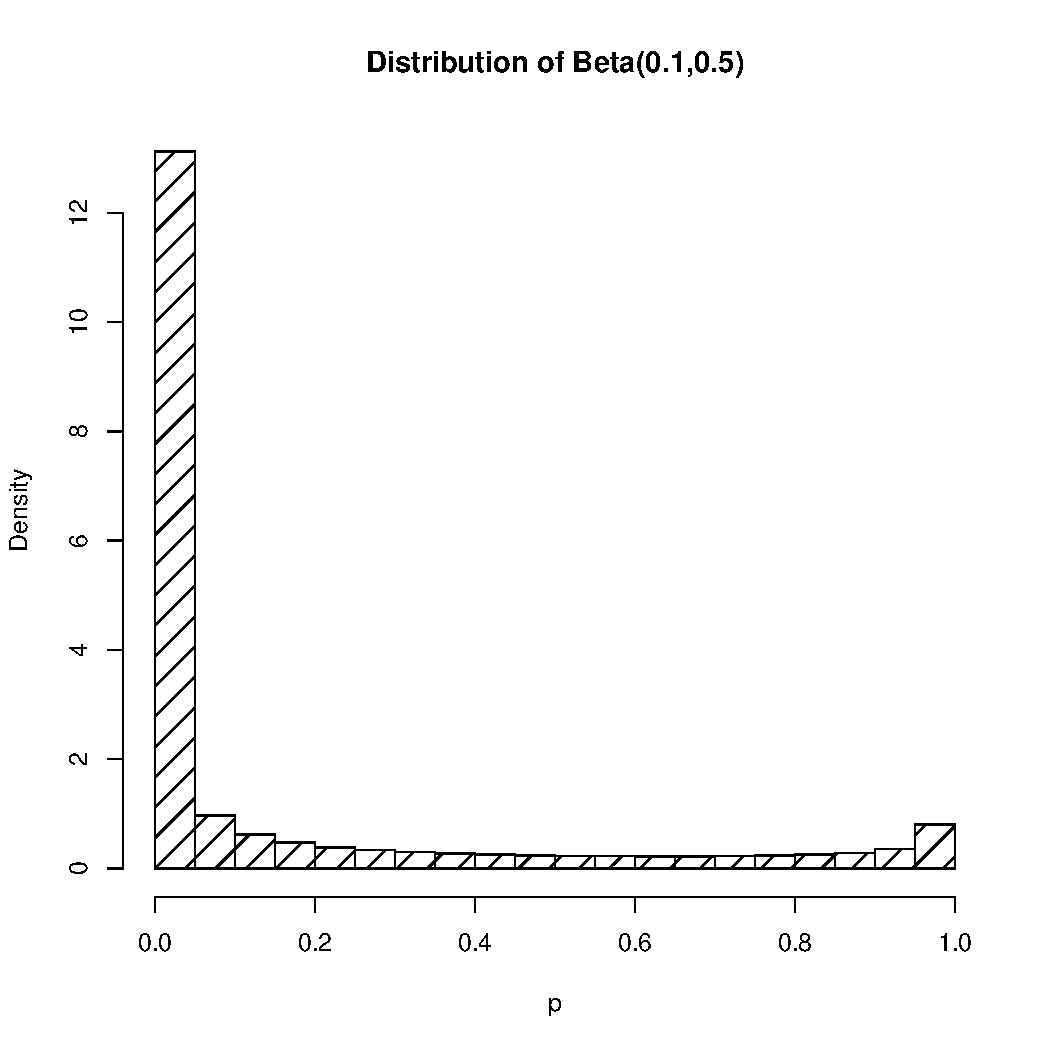
\includegraphics[width=.5\textwidth]{beta-dist}
  \caption{The distribution of users' page click rate parameter $p_i$ from $Beta(0.1,0.5)$ distribution.}
  \label{fig:beta-dist}
\end{figure}

We first test Formula X for page level metric $\xbar$. We  use page click rate (PCR) as an example. The page level measurement $X_{i,j}$ for page click rate is binary with 1 stands for clicked and 0 not clicked. Metrics with the exact same mathematical form includes ad click rate, ad coverage rate, etc. 

For a fixed $x$, each time, we sample a proportion $x$ of users as well as their $p_i$ from the $M$ users without replacement. Then we simulate the page view $K_i$ for each selected users from $Poisson(5)$. The rest of the simulation is straightforward, we simulate the number of page clicked by the user $i$ from $Binomial(K_i,p_i)$. For this simulated data, we then compute empirical PCR, $\naiveest$, $\deltaest$, and also apply Formula X in Theorem \ref{thm2.1}. On the other hand, to empirically estimate the true variance, we repeat this step for $1000$ times and calculate sample variances of the 1000 empirical PCRs. Note that for each of the $1000$ run we have an estimate from  $\naiveest$, $\deltaest$ and  Formula X. We take average of those $1000$ estimates respectively to represent the final output of $\naiveest$, $\deltaest$ and Formula X. The last step is to repeat the preceding step for a grid of $x$ varying from $0$ to $1$. We started with $x=0.02$ and linearly grow $x$ to $1$ with step size $0.02$. 

To test Formula X for user level metric $\wX$, we use the same page level measurement $X_{i,j}$ as above but roll up to user level. The simulation procedure is the same except for each fixed $x$, for each of the $1000$ simulation run we calculate $\wX$ and use the Formula X in Theorem \ref{thm2.2}. 
\begin{figure}[!htbp]
  \centering
  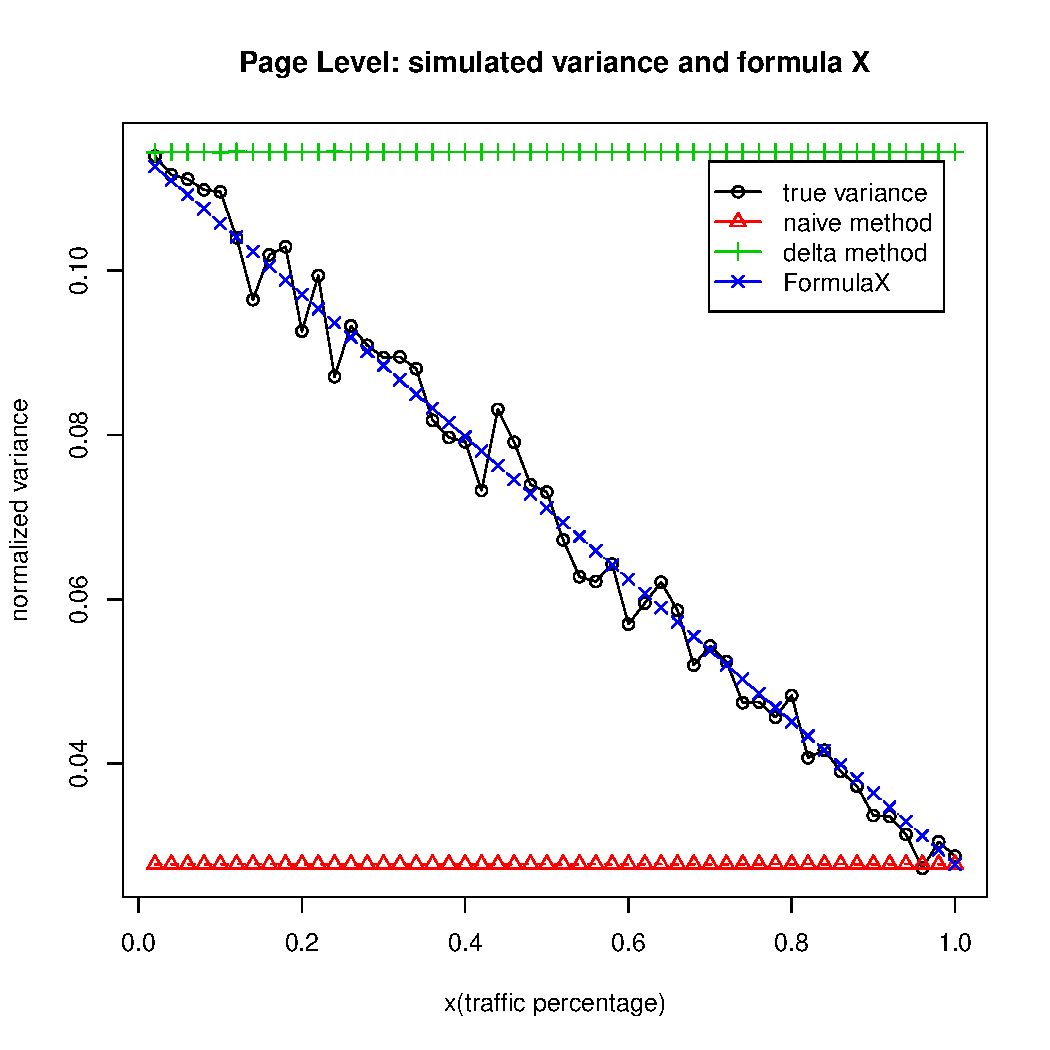
\includegraphics[width=0.49\textwidth]{pcr-kpois5}
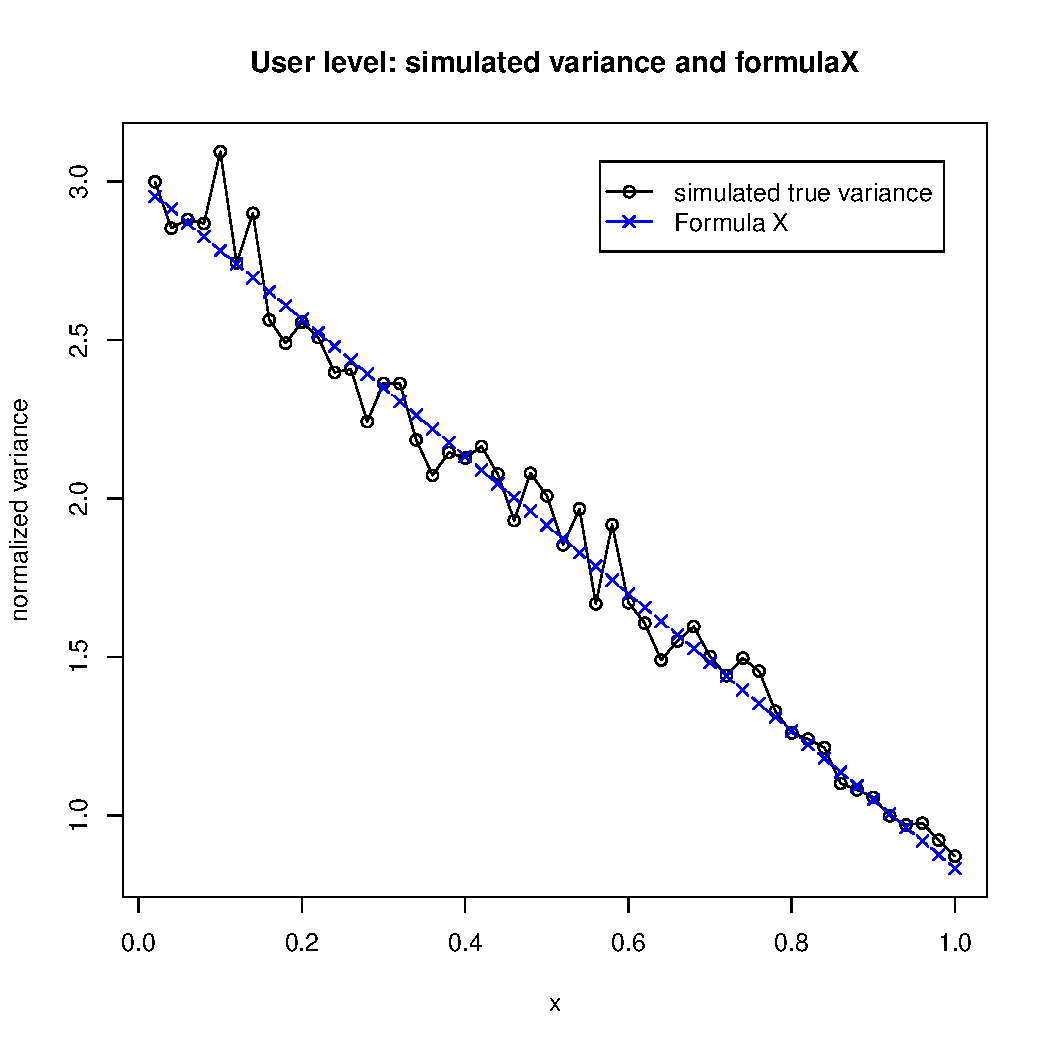
\includegraphics[width=0.49\textwidth]{usr-kpois5}
  \caption{Left: Plot of 3 estimators for normalized variances for $\xbar$ (naive method, delta method, Formula X) and the estimated true variances. The formula X predicts linearly decreasing variances as $x$ increase from $0$ to $1$. Right: Plot of the simulated variance of $\wX$(after normalization) and the estimated value from Formula X.}
  \label{fig:ctr-poisK}
\end{figure}
The results are summarized in Figure~\ref{fig:ctr-poisK}. The results show that Formula X performs quite well in both cases. The empirically estimated true normalized variance indeed varies around the value Formula X predicted. The prominent linearly decreasing trend agrees with Theorem \ref{thm2.1} and \ref{thm2.2}.



\section{Summary and Conclusions}\label{conclusion}
In this paper we showed, for both page level metrics and user level metrics, the limiting behavior of the normalized variance under the i.i.d assumptions(infinite user pool) and under the finite user pool model. Moreover, we gave consistent estimators for both type of metrics which in both cases is a linear function of $x$, the percentage of users sampled per group. Simulation studies supports the theoretical results and highlighted the decreasing trend of the true limiting variances  as $x$ increases. 

To see the implication of this finding, let's consider the page level metric $\xbar$.  For general controlled experiments, it is a natural and general practice to assume an infinite pool of users and based on this very assumption people treat users as independent even though we know each individual is a unique human being. The delta method is consistent if this assumption is right and a relatively common mistake people make is to use the naive formula which treats page level measurement as i.i.d.  But Formula X shows that if we assume a finite user pool and let $x$ goes to 1, the true normalized variances will decrease from the delta method estimate linearly to a smaller value that is closer to the estimate from the naive formula\footnote{In Figure \ref{fig:ctr-poisK}, it looks like Formula X gives approximately the same number as the naive formula (the triangle points), this is just a coincidence. But in general, it is safe to say that Formula X when $x$ goes to 1 gives a value that is much closer to the naive formula value than the delta formula value.}. The value of Formula X when $x$ equal to 1 is not exactly equal to the naive formula, but they are close for many cases and we can actually quantify it by comparing Theorem \ref{thm1.1} and \ref{thm2.1}.
Using delta method will only over-estimate the variance. Hence the type-I error will still get controlled. And when $x$ is close to 0, true variance and the delta method(or corresponding bootstrap estimates, if bootstrap user with replacement was used) are very close. So there is little gain of statistical power to actually use Formula X for the calculation of variance.
If $x=0.5$, the effect of using Formula X can really increase the power. For example, in the simulation study in Section \ref{simulation}, the normalized delta method variance is about 0.114, the true variance was estimated to be $0.071$. The true variance is about $62\%$ of the delta method estimate. How will this affect the statistical power?
Using the following  approximated relationship\footnote{Assume equal variance between control and treatment.} between power $\beta$, Type-I error $\alpha$, the coefficient variation, the expected percentage change (treatment effect) $\delta\%$ and the sample size $n_1$ and $n_2$ of two groups,
\begin{align}\label{power}
\frac{1}{1/n_1+1/n_2}= cv^2\Bigl(\frac{\Phi_{\alpha/2}+\Phi_\beta}{\delta\%}\Bigr)^2,
\end{align}  
if we further assume $n_1=n_2=n$ and $\delta\%$ fixed. Decreasing $CV^2$ by $62\%$ is equivalent to increasing sample size $n$ by $1/62\% = 1.61$. This is a significant gain because the experiments that we really need to allocate $50\%$ to a group in the first place are generally those that we suffer from low sample size. 

Theorem \ref{thm2.1} and \ref{thm2.2} assumes there is a static pool of users that the experiment designer want to make inference upon. It assumes we can collect data from all of them even if they didn't visit during the experiment and for these users by definition the number of page views $K_i$ is $0$. But in many cases, we are only interested in those users that are active, or at least have one visit during the experiment. More importantly,  if the user identification is based on cookie, based on the data collected during the experiment alone, we might not know there exists a user unless the user showed up at least once during the experiment. In Appendix \ref{practical}, we show a simple adjustment on Formula X can be made for this cases. Another dependency we didn't cover in this paper is that in the model of finite user pool, the metric for control and treatment groups $S_t$ and $S_c$ are no longer independent. But we believe this dependency is week and summing up Formula X estimates for control and treatment groups will be very close to the variance of $S_t-S_c$.


\subsection*{Acknowledgements}
The author wants to thank Roger Longbotham for the insightful discussion, consistent encouragement and support on this project. He also want to thank his colleague Ya Xu and Toby Walker for proposing this problem and their continuous help,  discussion and suggestion during the project.
\appendix
\appendixpage
\section{Adjustment for Inference on Active Users}\label{practical}
The results in Section \ref{finitecase} is quite general. For example, it allows $K_i$ to be 0, which means user $i$ had no page view during the experimentation. For web experimentation, if the user identification is based on cookie assignment, then when the user never came during the experiment, we might not know whether there exists such a user. In practice, many analysis was done on those users actually appeared in the experiment, \emph{i.e.}, with $K_i>0$. Theorem \ref{thm2.1} and \ref{thm2.2} can be easily adjusted for this case.

To see how the adjustment can be made for non user level metrics $\xbar$, assume that we know the appearance rate for a fixed duration of the experiment is $r$. There are many ways to estimate this rate, the web site owner can get the idea of the number of active users by counting the stable users for a relatively long period of time, months, for example. $r$ can be estimated by dividing the number of appeared users in the experiment by the total number of active users (scaled by the percentage of traffic that was allocated to the experiment). 

An important observation is that $\xbar$ can be calculated using only appeared users since those ``hidden'' users will have zero page views and zero $X_{i,j}$'s that will not contribute to $\xbar$. The only thing changes is the estimation of $\bbe K_i$ and $\bbe K_i^2$. Suppose $n_a$ is the number of users appeared, then the sample mean of $K_i$ and $K_i^2$ for those appeared users is actually unbiased estimator for $\wht{\bbe( K_i| K_i>0)}$ and $\wht{\bbe (K_i^2|K_i>0)}$. Simple algebra reveals that $\wht{\bbe K_i} = \wht{\bbe (K_i|K_i>0)}r$ and $\wht{\bbe K_i^2} = \wht{\bbe( K_i^2|K_i>0)}r$. Hence $C_a := \frac{\wht{\bbe( K_i^2|K_i>0)}}{ \wht{\bbe (K_i|K_i>0)}^2} = r \frac{\wht{\bbe K_i^2}}{\wht{\bbe K_i}^2} = r C$

If the analysis was done on those appeared users, then the normalized variance is defined as $n_a \var \xbar$. 
Therefore, from Theorem \ref{thm2.1},
\begin{align*}
n_a \var \xbar & = r\times n\var \xbar \to r\bigl\{(C- x) \var \mu_i + \bbe \sigma_i^2 / (\bbe(K_i|K_i>0)r)\bigr\}. \\
&= (C_a - xr) \var \mu_i + \bbe \sigma_i^2/ \bbe(K_i|K_i>0)
\end{align*}
Also, note that if we apply delta method or naive method on those appeared users, we are essentially conditioned on $K_i >0$ and we can estimate $\var (\mu_i|K_i>0)$ and $\bbe (\sigma_i^2|K_i>0)$ using \eqref{twoestimator} with the estimators all conditioned on $K_i >0$, \emph{i.e.}, use data from appeared users. Since $(\mu_i,\sigma_i^2)$ independent of $K_i$, this actually gives us consistent estimators of  $\var\mu_i$ and $\bbe \sigma_i^2$. In another word, we don't need to know these ``hidden'' users to estimate $\var\mu_i$ and $\bbe \sigma_i^2$.
The preceding argument shows that if we know the appearance rate $r$,  the only adjustment we need to make upon Theorem \ref{thm2.1} is that we need to replace $x$ to $rx$ and replace all other estimators by the conditioned version, \emph{i.e.}, using data from appeared users. The same argument applies to user level metric. Define $\wX_a=(\sum_{i=1}^{n_a}\sum_{j=1}^{K_i}X_{i,j})/n_a =( \sum_{i=1}^n \sum_{j=1}^{K_i})/n_a$ . It can be shown that 
\begin{align*}
	n_a \var \wX_a& \to  (\wht{\bbe( K_i^2|K_i>0)}- rx \wht{\bbe (K_i|K_i>0)}^2\wht{\var \mu_i} \\
&+ \wht{\bbe \mu_i}^2 \wht{\var (K_i|K_i>0)} + \wht{\bbe (K_i|K_i>0)} \wht{\bbe \sigma_i^2} .
\end{align*}

The intuition for the adjustments are that the ``effective'' sampling percentage is $xr$ rather than $x$. When the appearance rate $r$ is small, the finite user effect is again negligible because $xr$ is small. 

%An important observation is that under the assumption that $(\mu_i,\sigma_i^2)$ independent of $K_i$, $\bbe(\mu_i| K_i>0)$, $\bbe$

%
%\section* {References}
%
%\everypar = {\hangindent=0in \hangafter=1 }
%\smallskip \noindent
%Author, I. M. (1987),
%``,''
%{\em Some Fine Journal}, Vol. 17, pp. 1--100.
%
%\smallskip \noindent
%Expert, A. N. (1989),
%{\em A Book He Wrote,}
%His Publisher.

\bibliography{biblio}
\bibliographystyle{jmr}
\end{document}
